\documentclass[letterpaper]{article} % DO NOT CHANGE THIS
\usepackage[submission]{aaai2027} % DO NOT CHANGE THIS
\usepackage[hyphens]{url} % DO NOT CHANGE THIS
\usepackage{graphicx} % DO NOT CHANGE THIS
\urlstyle{rm} % DO NOT CHANGE THIS
\def\UrlFont{\rm} % DO NOT CHANGE THIS
\usepackage{natbib} % DO NOT CHANGE THIS AND DO NOT ADD ANY OPTIONS TO IT
\usepackage{caption} % DO NOT CHANGE THIS AND DO NOT ADD ANY OPTIONS TO IT
\usepackage{booktabs}
\usepackage{amsmath,amssymb,amsthm,mathtools}
\usepackage{microtype}
\usepackage{xcolor}
\frenchspacing % DO NOT CHANGE THIS

\pdfinfo{
/TemplateVersion (2027.1)
}

\newtheorem{definition}{Definition}
\newtheorem{theorem}{Theorem}
\newtheorem{proposition}{Proposition}
\newtheorem{corollary}{Corollary}
\newtheorem{lemma}{Lemma}
\theoremstyle{remark}
\newtheorem{remark}{Remark}

\newcommand{\cX}{\mathcal X}
\newcommand{\cZ}{\mathcal Z}
\newcommand{\cA}{\mathcal A}
\newcommand{\PiM}{\Pi_m}
\newcommand{\E}{\mathbb E}
\newcommand{\Pp}{\mathbb P}
\newcommand{\ind}{\mathbf 1}
\newcommand{\DRMS}{\textnormal{\textsc{DRMS}}}
\newcommand{\argmin}{\operatorname*{arg\,min}}
\newcommand{\argmax}{\operatorname*{arg\,max}}
\newcommand{\KL}{D_{\mathrm{KL}}}
\newcommand{\spanop}{\operatorname{span}}

\title{How Much History Is Enough?\\
Certifying Decision-Relevant Memory in Offline Reinforcement Learning}
\author{Anonymous Submission}
\affiliations{}

\begin{document}
\maketitle

\begin{abstract}
Partial observability is often handled by conditioning a policy on a fixed
window of recent observations and actions.  Longer windows can reveal hidden
state, but they also enlarge the effective state space and may retain history
that improves prediction without changing good decisions.  We study how to
select the shortest decision-sufficient history window from offline data.  In
a finite-horizon controlled process, candidate policies use suffixes of the
full observable history; importantly, these suffixes need not be Markov.  We
introduce a cellwise decision ambiguity: the minimum worst-case optimal
advantage loss incurred by applying one action distribution to full histories
sharing a suffix.  Zero ambiguity exactly characterizes the existence of an
optimal suffix policy, while cumulative ambiguity upper-bounds its uniform
value loss.  We then develop Decision-Relevant Memory Selection (\DRMS), which
converts simultaneous confidence intervals for the full-history optimal
\(Q\)-function into upper advantage costs and solves small cellwise linear
programs.  With high probability, \DRMS{} returns the shortest window whose
policy loss is certified below a chosen tolerance, without assuming that the
selected window is Markov.  We prove recovery under a separation condition and
matching upper and lower rates in a canonical family: memory identification
requires \(\Omega(\log(1/\delta)/(p\gamma^2))\) episodes when a decision
conflict occurs with probability \(p\) and action gap \(\gamma\).  Exact
tabular experiments separate next-observation prediction from
decision-relevant memory and recover the predicted coverage--gap scaling using
only lightweight CPU computation.
\end{abstract}

\section{Introduction}

An agent facing partial observability must decide what part of the past to
retain.  A common practical answer is frame stacking: concatenate a fixed
number of recent observations and actions, then apply an ordinary reinforcement
learning algorithm.  Choosing this window is consequential.  Too little
history aliases situations requiring different actions; too much history
inflates the effective state space, worsens offline coverage, and invites
spurious dependence on nuisance variables.  Recurrent policies avoid a fixed
window but introduce a larger architecture and tuning problem, and they do not
explain how much historical information the task actually requires.

A tempting solution is to select memory through prediction: retain history as
long as it improves prediction of the next observation or reward.  This tests
whether a truncated observation process is Markov, but the Markov property is
stronger than what control requires.  Two failures are possible.  First, an
old nuisance variable may remain highly predictive of future observations even
though it never changes the optimal action.  Prediction then over-prescribes
memory.  Second, an old cue may determine which action receives reward while
having no effect on subsequent observations.  A next-observation test then
under-prescribes memory.  Figure~\ref{fig:separation} gives exact instances of
both failures.

This paper asks a more direct question:

\begin{quote}
\emph{What is the shortest history window for which offline data can certify a
near-optimal policy?}
\end{quote}

We treat complete observable history as a finite-horizon MDP and compare nested
policy classes that use only an \(m\)-step suffix.  We never assume that
the suffix process is Markov.  Instead, we inspect whether histories merged by
the suffix can share an action without losing value.  This leads to a
population quantity defined from the full-history optimal advantages.  It is
zero exactly when a uniformly optimal \(m\)-memory policy exists, and it gives
an explicit approximation-error bound when exact sufficiency fails.

The population characterization becomes an offline certificate by replacing
unknown advantages with simultaneous upper confidence bounds.  Each suffix
cell requires only a small minimax linear program.  The resulting procedure,
\DRMS, either returns a short policy with a high-confidence value-loss bound or
abstains when the data do not support one.  Since the guarantee is simultaneous
across memory lengths, the same data can be used to choose the window without
invalid post-selection reasoning.

Our main contributions are:
\begin{itemize}
  \item We define \emph{decision ambiguity} for temporal suffix classes and
  prove monotonicity, an exact decision-sufficiency characterization, and a
  value-loss sandwich.
  \item We show that next-observation predictive diagnostics and
  decision-relevant memory are incomparable: either can demand arbitrarily
  longer history than the other.
  \item We introduce \DRMS, an interval-based offline certifier that remains
  valid even though the selected short history is non-Markov.
  \item We prove exact-memory recovery under an advantage separation and
  matching upper and lower rates of order \(1/(p\gamma^2)\) in a canonical
  rare-context family.
  \item We provide transparent tabular code and theorem-driven experiments.
  Across 12 coverage--gap settings, the empirical episodes needed for 50\%
  recovery scale with \(1/(p\gamma^2)\) with log--log slope \(0.94\).
\end{itemize}

\section{Related Work}

\paragraph{Memory and partial observability.}
General POMDP planning can require a belief over latent states
\citep{kaelbling1998pomdp}.  Known-model analyses bound finite-window
approximation under nonlinear-filter stability \citep{kara2022finite}, while
short-memory POMDP theory assumes that a recent window decodes latent state and
obtains complexity depending on the window length rather than the full horizon
\citep{efroni2022short}.  Recent metric belief approximation gives
policy-conditional finite-memory loss bounds \citep{kim2026belief}.  Offline
POMDP learning has been studied through finite-memory Bellman operators and
structural assumptions such as undercompleteness \citep{guo2022offlinepomdp},
and offline safe policy improvement with finite-state controllers assumes a
fixed memory structure \citep{simao2023safe}.  Memory traces provide a compact
alternative to raw windows and yield offline on-policy evaluation guarantees
\citep{eberhard2025traces}; recurrent model-free policies can also be strong
empirical POMDP baselines \citep{ni2022recurrent}.  These works ask how to
learn or improve a policy with a specified memory mechanism.  We instead
select among nested raw-history suffixes from fixed data and certify decision
loss without requiring the selected suffix to be Markov.

\paragraph{Prediction and state representation.}
Predictive-state ideas represent history through forecasts of future events
\citep{littman2001predictive}.  Recent Markov Violation Scores diagnose
non-Markov observations by testing whether history reduces prediction error
\citep{mysore2026mvs}.  Our counterexamples show why next-observation
predictive violation is not itself a policy-memory criterion.  The broader
state-abstraction literature characterizes value- and policy-preserving
mappings \citep{li2006unified,abel2016approximate,abel2020value}, and
action-sufficient representation
learning targets variables needed for control \citep{huang2022action}.  We
specialize decision sufficiency to temporal suffix partitions and add offline
selection, confidence certification, and coverage-dependent lower bounds.

\paragraph{Offline RL and model selection.}
Offline RL uses pessimism to avoid unsupported decisions
\citep{jin2021pessimism,shi2022pessimistic}.  Related work connects pessimistic
offline RL with imitation learning \citep{rashidinejad2021bridging}.
ModBE selects among nested value-function classes using oracle inequalities
\citep{lee2022oracle}.  Our nested objects are policy information sets rather
than Bellman model classes: a shorter suffix may be non-Markov and Bellman
incomplete yet still contain an optimal policy.  We use full-history
confidence intervals only to certify the action compromises induced by each
suffix partition.

\section{Setting and Objective}

Consider a finite-horizon controlled process with stages \(h\in[H]\), bounded
rewards \(R_h\in[0,1]\), and finite action sets \(\cA_h\).  Let
\(X_h\in\cX_h\) be the complete observable action--observation history before
action \(A_h\).  The complete history is a valid Markov state, with reward
mean \(r_h(x,a)\) and transition kernel \(P_h(\cdot\mid x,a)\).  Let
\(Q_h^*,V_h^*\) be the corresponding optimal action-value and value functions.

For memory length \(m\), the map \(\phi_{m,h}(x)\) retains the latest \(m\)
observations and intervening actions, or all available history when \(h<m\).
A policy belongs to
\[
\Pi_m=\{\pi:\pi_h(\cdot\mid x)=\pi_h(\cdot\mid\phi_{m,h}(x))\}.
\]
The classes are nested.  We emphasize that \(Z_h=\phi_{m,h}(X_h)\) need not be
Markov for \(m<H\).

We seek the shortest \(m\) supporting small uniform loss.  Define
\[
\mathcal E_m
=\inf_{\pi\in\Pi_m}\max_{h,x}
\bigl[V_h^*(x)-V_h^\pi(x)\bigr].
\]
We use uniform loss for a clean distribution-free theory and defer
occupancy weighting to the limitations.

\section{Decision-Relevant Memory}

Define the optimal advantage loss
\[
A_h^*(x,a)=V_h^*(x)-Q_h^*(x,a)\geq0.
\]
For suffix \(z\), let
\(C_{m,h}(z)=\{x:\phi_{m,h}(x)=z\}\) be the full histories that an
\(m\)-memory policy must treat identically.

\begin{definition}[Decision ambiguity]
The ambiguity of one suffix cell is
\[
\eta_{m,h}(z)=
\min_{p\in\Delta(\cA_h)}
\max_{x\in C_{m,h}(z)}
\E_{a\sim p}A_h^*(x,a).
\]
Let \(\eta_{m,h}=\max_z\eta_{m,h}(z)\) and
\(G_m=\sum_{h=1}^H\eta_{m,h}\).
\end{definition}

The inner policy is allowed to randomize.  For deterministic policies, zero
ambiguity means that every suffix cell has a common optimal action.  The
quantity is computable by a linear program with \(|\cA_h|+1\) variables per
cell.

\begin{theorem}[Population characterization]\label{thm:population}
For every \(m\):
\begin{enumerate}
  \item \(G_{m+1}\leq G_m\).
  \item \(G_m=0\) if and only if there exists
  \(\pi\in\Pi_m\) with \(V_h^\pi(x)=V_h^*(x)\) for every \(h,x\).
  \item The best attainable uniform loss satisfies
  \[
  \max_h\eta_{m,h}\leq\mathcal E_m\leq G_m.
  \]
\end{enumerate}
The cellwise minimax policy \(\pi^m\) additionally obeys
\[
V_h^*(x)-V_h^{\pi^m}(x)
\leq\sum_{t=h}^H\eta_{m,t}.
\]
\end{theorem}

The proof uses no Markov property for the suffix.  For the upper bound, let
\(D_h(x)=V_h^*(x)-V_h^{\pi^m}(x)\).  Adding and subtracting the full-history
optimal continuation gives
\[
\begin{aligned}
D_h(x)
&=\E_{a\sim\pi_h^m}A_h^*(x,a)\\
&\quad +\E_{a,X'}D_{h+1}(X')\\
&\leq\eta_{m,h}+\|D_{h+1}\|_\infty.
\end{aligned}
\]
Backward induction proves the claim.  Conversely, any suffix policy must use
one action distribution throughout a cell, while replacing its continuation
by \(V^*\) can only increase value; this yields the lower bound.  Full proofs
are in the supplement.

For a behavior policy \(\mu\), write \(Z_h^m=\phi_{m,h}(X_h)\) and define
the oracle next-observation residual
\[
\begin{aligned}
R_m^{\rm obs}
&=\sum_h H_\mu(O_{h+1}\mid Z_h^m,A_h)\\
&\quad-\sum_h H_\mu(O_{h+1}\mid X_h,A_h).
\end{aligned}
\]
This mirrors observation-prediction diagnostics, not the full controlled Markov
condition.  If the conditional joint law of reward and next suffix is identical
within every suffix cell for every action, then an optimal suffix policy exists
and \(G_m=0\).

\begin{figure*}[t]
  \centering
  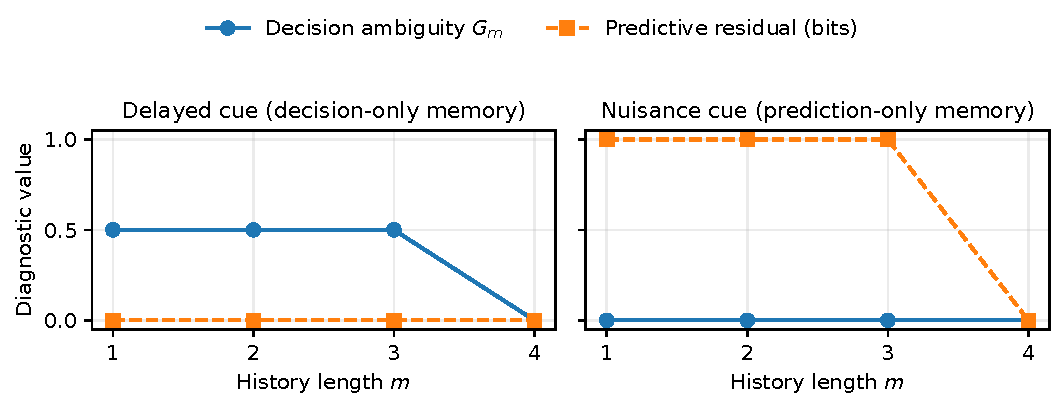
\includegraphics[width=0.93\textwidth]{../figures/decision_vs_prediction.pdf}
  \caption{\textbf{Next-observation prediction and decision-relevant memory
  can disagree in both directions.}  In the delayed-cue task (left), a
  stage-one cue determines the final rewarding action, but future observations
  are constant: \(R_m^{\rm obs}=0\), whereas \(G_m=1/2\) until the cue enters
  the suffix.  In the nuisance task (right), the cue predicts the terminal
  observation but never changes the optimal action, so \(G_m=0\) at every
  memory length.  Values are exact for \(H=4\) and a balanced binary cue.}
  \label{fig:separation}
\end{figure*}

\begin{proposition}[Observation-prediction separation]\label{prop:separation}
For any horizon \(H\), there are controlled processes under a uniform behavior
policy in which: (i) \(R_m^{\rm obs}=0\) for every \(m\), but
\(G_m=\gamma/2\) for all \(m<H\) and \(G_H=0\); and (ii) \(G_m=0\) for
every \(m\), but \(R_m^{\rm obs}=1\) bit for all \(m<H\).  Thus an
observation-prediction diagnostic can require arbitrarily more or less history
than decision sufficiency.
\end{proposition}

\section{Offline Certification with \DRMS}

Assume an offline procedure produces simultaneous intervals
\[
L_h(x,a)\leq Q_h^*(x,a)\leq U_h(x,a)
\quad\text{for all }h,x,a
\tag{1}\label{eq:qevent}
\]
with probability at least \(1-\delta\).  Our core result is modular: any valid
full-history \(Q^*\) intervals may be used.

A naive upper advantage, \(\max_b U_h(x,b)-L_h(x,a)\), is unnecessarily loose
because comparing action \(a\) with itself has exactly zero loss.  We instead
define
\[
\overline A_h(x,a)=
\max\left\{0,\max_{b\neq a}[U_h(x,b)-L_h(x,a)]\right\},
\tag{2}\label{eq:upperadv}
\]
with \(\overline A_h=0\) at one-action stages.  On event~\eqref{eq:qevent},
\(A_h^*(x,a)\leq\overline A_h(x,a)\).

Replace \(A_h^*\) by \(\overline A_h\) in Definition~1 to obtain robust
ambiguities \(\overline\eta_{m,h}(z)\) and
\(\overline G_m=\sum_h\max_z\overline\eta_{m,h}(z)\), along with the robust
cellwise policy \(\overline\pi^m\).

\paragraph{Decision-Relevant Memory Selection.}
Given tolerance \(\epsilon\), \DRMS{} performs:
\begin{enumerate}
  \item estimate simultaneous full-history intervals \((L,U)\);
  \item for each \(m,h,z\), solve the minimax LP using costs
  \(\overline A_h\);
  \item return the smallest \(m\) with \(\overline G_m\leq\epsilon\) and its
  policy \(\overline\pi^m\);
  \item if no candidate passes, return the longest candidate with an explicit
  abstention flag.
\end{enumerate}

\begin{theorem}[High-confidence value certificate]\label{thm:certificate}
On event~\eqref{eq:qevent}, simultaneously for every memory length \(m\),
\[
V_h^*(x)-V_h^{\overline\pi^m}(x)
\leq\sum_{t=h}^H\overline\eta_{m,t}
\quad\text{for all }h,x.
\]
Consequently, whenever \DRMS{} certifies
\(\overline G_{\widehat m}\leq\epsilon\), its selected policy has uniform
value loss at most \(\epsilon\).
\end{theorem}

The theorem follows by the same backward recursion as
Theorem~\ref{thm:population}, now using
\(A_h^*\leq\overline A_h\).  Since the intervals are simultaneous, the result
holds for the data-selected memory without a second holdout set.

\begin{proposition}[Tightness and recovery]\label{prop:tightness}
Suppose every interval has one-sided error at most \(w\).  Then
\[
G_m\leq\overline G_m\leq G_m+2Hw.
\]
If \(m_{\rm dec}=\min\{m:G_m=0\}>1\), let
\(\Gamma=\min_{m<m_{\rm dec}}G_m\).  If \(2Hw<\Gamma\), every threshold
\(\epsilon\in[2Hw,\Gamma)\) makes \DRMS{} recover \(m_{\rm dec}\).
\end{proposition}

This yields a certificate--complexity tradeoff: longer memory weakly
decreases ambiguity, while \DRMS{} returns the shortest window meeting a
user-specified loss budget.  Statistical uncertainty is inherited from the
common full-history confidence set.  The present method therefore certifies
memory parsimony rather than balancing separately estimated models.

\section{Tabular Instantiation and Statistical Limit}

For transparency, we instantiate Eq.~\eqref{eq:qevent} in a finite
full-history MDP from \(n\) independent behavior-policy episodes.  For each
\((h,x,a)\), empirical rewards use a union-bounded Hoeffding radius, and
empirical transitions use an \(L_1\) radius based on
\citet{weissman2003l1}.  Optimistic and pessimistic dynamic programming
propagate these model intervals using
\[
|(P-\widehat P)^\top f|
\leq\tfrac12\|P-\widehat P\|_1\spanop(f).
\]
A backward induction gives simultaneous \(Q^*\) coverage.  Unobserved pairs
receive the full reward radius and transition radius two; therefore the method
abstains rather than extrapolating through unsupported histories.

Coverage is not merely an artifact of our algorithm.  The following lower
bound identifies the intrinsic difficulty of deciding whether an old cue is
needed.

\begin{theorem}[Memory-order lower bound]\label{thm:lower}
Fix \(0<p<1\), \(0<\gamma\leq1/2\), and \(0<\delta<1/4\).  There are two
horizon-two processes observed under the same uniform behavior policy such
that their shortest decision-sufficient memories are one and two,
respectively, and any estimator that identifies the correct memory with error
at most \(\delta\) on both requires
\[
 n\geq \frac{\log(1/(4\delta))}{6p\gamma^2}.
\]
\end{theorem}

In the construction, a cue is rare with probability \(p\).  In the first
model, action zero is better by \(\gamma\) after either cue.  In the second,
the optimal action flips only after the rare cue.  The one-episode KL
divergence is at most \(6p\gamma^2\), and the result follows from the
Bretagnolle--Huber inequality \citep{tsybakov2009nonparametric}.  The theorem
explains why memory selection is hard precisely when decision-conflicting
histories are rare or their action gaps are small.

\begin{corollary}[Matching upper rate in the two-point family]\label{cor:upper}
Let \(p\leq1/2\), and let \(M\) be the number of full-history
state--action pairs.  Tabular \DRMS{} with tolerance \(\gamma/4\) and
confidence level \(\delta/2\) recovers the correct memory in both models with
probability at least \(1-\delta\) whenever
\[
n\geq \frac{32\log(8M/\delta)}{p\gamma^2}.
\]
\end{corollary}
The proof combines a binomial lower tail for every final state--action count
with reward confidence radii small enough to separate the two actions.  Thus
the lower bound is tight in \(p\) and \(\gamma\), up to logarithms and constants.

\section{Experiments}

Our experiments are deliberately small: their role is to validate theorem
predictions, not to claim deep-control state of the art.  All values in the
population study are computed exactly.  Finite-sample runs use only tabular
counts, dynamic programming, and two-action cellwise minimax solutions.

\paragraph{Prediction can select the wrong memory in both directions.}
Figure~\ref{fig:separation} uses horizon four.  In the delayed-cue process, the
cue leaves the suffix until \(m=4\); a memoryless final action incurs minimax
loss \(1/2\), while the next observation is always deterministic.  In the
nuisance process, the cue contributes one bit of terminal predictive
information but action zero is optimal for both cues.  The computed policy
loss equals \(G_m\) in both examples.

\paragraph{Tolerance adapts to decision relevance.}
We vary the delayed-cue reward gap \(\gamma\) at horizon five.  Every
insufficient suffix has population ambiguity \(\gamma/2\), so tolerance
\(\epsilon\) should select memory one exactly when
\(\gamma\leq2\epsilon\), and full memory otherwise.  The implementation
recovers these four phase transitions exactly; the corresponding plot is in
the supplement.

\begin{figure*}[t]
  \centering
  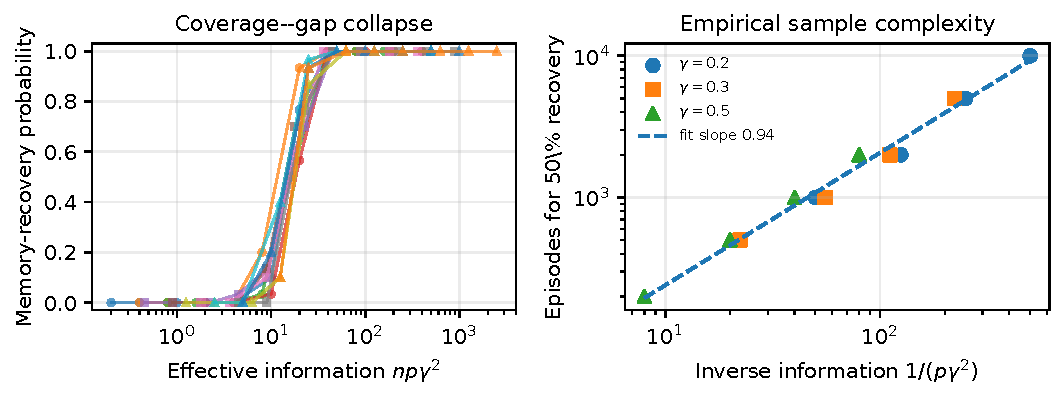
\includegraphics[width=0.94\textwidth]{../figures/coverage_gap_scaling.pdf}
  \caption{\textbf{Finite-sample behavior follows the information-theoretic
  scaling.}  We vary rare-cue probability
  \(p\in\{0.05,0.1,0.2,0.5\}\), action gap
  \(\gamma\in\{0.2,0.3,0.5\}\), and eight dataset sizes, with 30 seeds per
  point.  The tolerance is \(\gamma/4\).  Left: all 12 recovery curves nearly
  collapse against \(np\gamma^2\).  Right: the first grid size attaining at
  least 50\% correct certification is approximately linear in
  \(1/(p\gamma^2)\); the fitted log--log slope is 0.94.}
  \label{fig:scaling}
\end{figure*}

\paragraph{Coverage--gap scaling and calibration.}
Figure~\ref{fig:scaling} evaluates the matching dependence in
Theorem~\ref{thm:lower} and Corollary~\ref{cor:upper}.  We run 2,880 independent datasets over 12
\((p,\gamma)\) combinations.  The empirical 50\%-recovery threshold has a
log--log slope of 0.935 against \(1/(p\gamma^2)\).  In a separate calibration
sweep with 1,600 datasets, four values of \(p\), and fixed
\(\gamma=0.5,\epsilon=0.1\), simultaneous \(Q\)-interval coverage and policy
certificate validity are both 100\%; no run falsely certifies a shorter
memory.  These observations are sanity checks rather than substitutes for the
finite-sample theorem, but they show that the conservative construction becomes
informative at the predicted effective sample scale.

\paragraph{Reproducibility.}
The entire experiment suite runs on CPU.  The repository includes exact MDP
constructors, interval dynamic programming, cellwise solvers, raw and summary
CSVs, figure scripts, and unit tests.  The main scaling experiment uses 30
seeds; all configuration values are encoded in the scripts.

\section{Limitations and Conclusion}

The present theory enumerates a known finite maximum history and uses uniform
loss over all feasible full contexts.  This is intentionally conservative:
long histories can be exponentially numerous, and a rare but irrelevant
context can block certification.  The next theoretical step is an
occupancy-weighted ambiguity with a concentrability-based value guarantee.
Function approximation, continuous observations, and jointly learning a
representation and its memory length remain open.  Our tabular confidence set
is also designed for transparency rather than sharp constants.

Within this scope, the results establish a simple principle: memory should be
selected according to the action regret created by forgetting, not according
to prediction alone.  Decision ambiguity makes that principle exact at the
population level, while \DRMS{} turns it into an offline, high-confidence
certificate that can abstain when coverage is inadequate.  The matching-form
coverage--gap lower bound clarifies when such certification is statistically
possible.

\bibliography{references}

\end{document}
